% Tell Texshop where the project root is
%!TEX root = requirements.tex
%
\subsection{Sorption}  \label{sec:Sorption}

\subsubsection{Overview} 

Sorption involves the attachment of dissolved and/or colloidal species to mineral or other solid surfaces.  Sorption has the effect of slowing the effective transport rate of a species through porous media through its retardation effect.  The retardation effect for a species, $R_f$, is given by~\citep{bouwer-1991}
\begin{equation}
  R_f = \frac{V_{gw}}{V_{sp}},
\end{equation}
where 
$V_{gw}$ is the velocity of the groundwater and $V_{sp}$ is the velocity of the species.  
A variety of models have been used to describe sorption and can be broadly divided 
into those that describe it as a bulk process versus those that are mineral or solid phase specific.  
The latter approach involves the calculation of  bulk sorption from the sum of sorption on individual solid phases, 
an assumption referred to as \textit{Component Additivity}.  
Within the class of bulk sorption models, a distinction can be made between those 
which assume a finite number of sorption sites (these are referred to as showing 
Langmuir type behavior and include the Langmuir isotherm itself and most surface complexation 
and ion exchange models) and those that assume either an infinite sorption capacity 
or at least a capacity that is not tightly constrained 
(these include the linear distribution coefficient and the nonlinear Freundlich isotherm).  
Alternatively, one could also distinguish between single component, 
non-competitive models (e.g., Langmuir and Freundlich) and multicomponent competitive models (surface complexation and ion exchange).

Another possible distinction is between equilibrium and kinetic sorption models.  
In many cases, the formulations for the equilibrium and kinetic cases differ 
only insofar as the kinetic case involves involves a thermodynamic driving force 
(as in the equilibrium case), but modified by a finite rate constant.  
In some cases, however, sorption is described as irreversible, which implies that there is no back reaction (desorption).

%%\paragraph{Assumptions, Approximations, Applicability.}


\subsubsection{Process Model Equations}

\paragraph{Linear Distribution Coefficients ($K_d$).}
A simple approach to describe metal or ionic radionuclide sorption by a sediment,
\begin{equation}
  A_{aq}\leftrightharpoons A_{ads},
\end{equation}
is to use a constant distribution coefficient, defined by:
\begin{equation} \label{eq:Kd} 
  K_d = \frac{[A_{ads}]}{[A_{aq}]},
\end{equation} 
where $K_d$ is the distribution coefficient (L/kg), $[A_{ads}]$ is the sorbed concentration (mol/kg) to the bulk solid phase, 
and $[A_{aq}]$ is the total dissolved concentration in groundwater (mol/L) \citep{davis-1990}.  
One of the key advantages of representing sorption with a distribution coefficient is that it can be easily incorporated 
into reactive transport models used for migration predictions. 

Equation \eqref{eq:Kd} shows that if one assumes that the amount of sorption is proportional to the dissolved concentration, 
then there is a linear relationship where the $K_d$ value is the slope. 
In this simple case, referred to as a linear isotherm, retardation of a concentration  front in simple porous media is given by
%
\begin{equation}  \label{eq:KdRetardation}
  \frac{\bar{v}}{\bar{v}_{c} } 
  =
  1+\frac{\rho _{b} }{n} K_{d}  ,
\end{equation}
where $\rho_b$ is the bulk density, 
$n$ the porosity, 
$\bar{v}$ the average linear velocity of the groundwater and 
$\bar{v}_{c} $ the velocity of the point on the concentration profile 
where the concentration is half that of the input concentration \citep{freeze-1979}. 
Note that the ratio $\bar{v}$/$\bar{v}_{c} $ here is the retardation factor and represents 
the retardation of the movement of front relative to the flowing groundwater. 
While this is a simplified example, it serves to illustrate the key point that the $K_d$ value 
directly influences predictions of adsorbing metal or radionuclide mobility. 

%Could have the following
\subparagraph{Assumptions and Applicability} 
Sorption is proportional to the dissolved concentration. 
The aqueous and adsorbed phases are in equilibrium.

\subparagraph{Data Needs}
Typically $K_d$ values are determined for a particular subsurface material 
from the slope of a fitted line to the concentration of the sorbed species, $A_{ads}$, 
plotted versus the dissolved concentration of the same species, $A_{aq}$.  
These data may be derived from laboratory analyses, where one typically varies the dissolved concentrations systematically, 
or they may be derived from in situ field data.  
Since $K_d$ values may be variable, and in particular a function of temperature, 
pH or the redox state of the system (see below), it is often necessary to compile them in a lookup table for use by a particular computer code.

\paragraph{Langmuir Isotherm.}
The Langmuir isotherm assumes that the sorption sites, S, on the surface of a solid (absorbent) become occupied 
by an absorbate from the solution, A.  Implying a 1:1 stoichiometry
%
\begin{equation}  \label{eq:langmuir} 
  S + A \leftrightharpoons SA,
\end{equation}
where $SA$ is the adsorbed species on the surface. At equilibrium, a
standard mass action equation can be written:
%
\begin{equation}  \label{eq:langmuir_massaction}
  K_{ads,L} = \frac{ [ SA ] }{ [S] \{A\} },
\end{equation}
where the square brackets here refer to the concentration of the
species or site, and the curly brackets refer to the aqueous
activity.  Using the maximum concentration of surface sites, $S_T$
%
\begin{equation}  \label{eq:totalsurfacesites}
  [S_T] = [S] + [SA],
\end{equation}
one can write the Langmuir isotherm in its familiar hyperbolic form
%
\begin{equation}  \label{eq:hyperbolicLangmuir}
  [SA] = [S_T] \frac{ K_{ads} \{A\} }{1 + K_{ads} \{A\} }.
\end{equation}

%Could have the following
\subparagraph{Assumptions} 
For the following, it is assumed that the surface and aqueous species are in equilibrium.

\subparagraph{Data Needs} 
The equilbrium constant, $K_{ads}$, is typically obtained from experimental data. 
It depends on the specified absorbent and absorbate, and may be a function of temperature. 
It may be calculated from:
\begin{equation}
  K_{ads} = \exp\left(\frac{-\Delta G^{\circ}_{ads}}{RT}\right),
\end{equation}
where $\Delta G$ is the change in free energy for the reaction,
typically obtained from a database, $R$ is the gas constant and $T$ is the temperature.

\paragraph{Freundlich.} 
The Freundlich isotherm is another equilibrium model for sorption of absorabte A onto sorption sites, S
\begin{equation}  \label{eq:langmuir_reaction} 
  S + A \leftrightharpoons SA.
\end{equation}
Represented by the mass action equation:
\begin{equation}
  K_{ads,F} = \frac{ [ SA ] }{ \{A\}^{\beta_F} },
\end{equation}
where the square brackets again refer to the concentration of the
species or site, the curly brackets refer to the aqueous activity.
$K_{ads,F}$ and ${\beta_F}$ are the Freundlich parameters
\citep[e.g.][]{langmuir-1997, stumm-1992}.

%Could have the following
\subparagraph{Assumptions} 
For the following, it is assumed that the surface and aqueous species are in equilibrium.

\subparagraph{Data Needs} 
The Freundlich parameters, $K_{ads,F}$ and $n$, are generally obtained by fits to experimental data 
for a specific surface and aqueous species. 
They will generally be obtained from a database, and 
may be represented by a functional form or lookup table.

%Steefel
\paragraph{Multi-site, Multi-component Ion Exchange.}
An ion exchange reaction can be described via a mass action expression
with an associated equilibrium constant \citep{vanselow-1932,sposito-1981,appelo-1993}.  
The exchange reaction can be written in generic form as
\begin{equation}
  vACl_{u} (aq)+uBX_{\nu } (s)\leftrightharpoons uBCl_{\nu } (aq)+vAX_{u} (s),
\end{equation} 
where X refers to the exchange site occupied by the cations $A^{u+}$ and $B^{v+}$.  
The equilibrium constant, $K_{eq}$, for this reaction can be written as \citep{vanselow-1932}
\begin{equation}
  K_{eq} =\frac{\{BCl_{\nu } \}^{u} \{AX_{u}\}^{\nu } }{\{ACl_{u} \}^{\nu } \{BX_{\nu } \}^{u} },
\end{equation} 
where the curly braces refer to the thermodynamic activities.
Several activity conventions are in wide use.  One possibility is the
Gaines-Thomas activity convention, which assumes a reaction
stoichiometry of the following form \citep{appelo-1993}, written
here assuming the $Cs^+$ is the relevant cation of interest
\begin{equation}
  Cs^{+} + (1/z) MX(i)_{z} \leftrightharpoons CsX(i) + (1/z) M^{z+},
\end{equation} 
where $M$ is the competing cation ($Na^+$, $K^+$, $Ca^{++}$), $z$ is
its charge, and $X(i)$ refers to the $i^{th}$ type of exchange site.  
In the Gaines-Thomas convention, each exchange site, $X(i)$ has a charge of -1. 
The activities of adsorbed species correspond to the charge equivalent fractions, $\beta (i)_{M} $,
\begin{equation}
  \beta (i)_{M} =\frac{z_{M} q(i)_{M} }{\sum _{M}z_{M} q(i)_{M}  } = \{X(i)_{M} \},
\end{equation} 
where $z_M$ is the charge of cation $M$, $q(i)_M$ is the concentration
of adsorbed cation $M$ in exchange site \textit{i} (moles/g),
and the curly brackets denote activities.  
The Gapon activity convention is obtained by writing the reactions in every case with a
single exchanger \citep{appelo-1993}.  
Alternatively, the Vanselow convention \citep{vanselow-1932} describes the exchanger activity
with mole fractions
\begin{equation}
  \beta (i)_{M} =\frac{q(i)_{M} }{\sum _{M}q(i)_{M}  } = \{ X(i)_{M} \}.
\end{equation} 
The exchange reactions can then be used to write a mass action equation for binary Cs-M exchange:
\begin{eqnarray}
  K_{M/Cs} & = & \frac{\beta (i)_{M} ^{1/z} \{Cs^{+} \}}{\beta (i)_{Cs} \{M^{z+} \}^{1/z} } \\
  & = & 
\frac{\{X(i)_{M} \}^{1/z} \{Cs^{+} \}}{\{X(i)_{Cs} \}\{M^{z+} \}^{1/z} } .
\end{eqnarray}

In a single-site ion exchange model, the CEC is equal to the sum of the charge equivalent concentrations of the adsorbed cations:
\begin{equation}
  CEC = \sum _{M}z_{M} q_{M},
\end{equation} 
while in a multi-site model, the CEC is the charge summed over all of the cation exchange sites \citep{cernik-1996, voegelin-2000}
\begin{equation}
  CEC = \sum _{i}\sum _{M}z_{M} q(i)_{M}   .
\end{equation} 

%Could have the following
\subparagraph{Assumptions} 
For the following, it is assumed that the surface and aqueous species are in equilibrium.
%\todo{Need short description here}

%%\subparagraph{Data Needs}
%%\todo{Need short description here}

\paragraph{Surface Complexation.} 
\label{sec:surfaceComplexation} An alternative approach that allows a modeler to describe sorption while
simultaneously considering variable chemical conditions in the subsurface is a surface complexation model \citep{davis-2004}.  
In this approach, the sorbing sediment surfaces are considered to possess
surface functional groups that can form complexes analogous to the
formation of aqueous complexes in solution.  
These surface reactions include proton exchange, cation binding and anion binding via ligand
exchange at surface hydroxil sites (represented here as $XOH$ to avoid
confusion with other chemical species). 
For example, the sorption of a metal could be represented as
%
\begin{equation} \label{eq:metalSorption} 
  XOH + M^{z_+} \leftrightharpoons XOM^{z_+ - 1} + H^{+}  .
\end{equation} 

At equilibrium, the sorption reactions can be described by the mass law equation
%
\begin{equation} \label{eq:sorptionMassAction}
  K_{app} =\frac{\left[XOM^{z_{+}-1 } \right]\{H^{+} \} }{\left[XOH\right] \{M^{z+} \} }  ,
\end{equation} 
where $K_{app}$ is referred to as the apparent equilibrium constant,
because it includes surface charge effects and hence is dependent on
the extent of surface ionization \citep{dzombak-1990}, $\{i\}$
is the thermodynamic activity of aqueous species $i$, and the terms in
square brackets represent the concentration of surface complexes (mol/kg).

Surface complexation differs from the simpler isotherm and
ion-exchange models in several important ways. Surface complexation is
based on the electrical double layer (EDL) theory. EDL theory assumes
that the surface charge of a sorbent in contact with solution
generates an electrostatic potential that declines rapidly away from
the sorbent surface, creating an electrostatic field. An additional
energetic term accounting for the work needed for the aqueous species
to travel across the surface electric field is required:
%
\begin{eqnarray} \label{eq:EDLdeltaG}
\Delta G_{ads} & = & \Delta G_{intr} + \Delta G_{coul} \nonumber \\
               & = & \Delta G_{intr} + (\Delta G_{\psi =0} - \Delta G_{\psi =\psi_{0} } ) \nonumber \\
               & = & \Delta G_{intr} - z F \psi_{0}  .
\end{eqnarray} 
\noindent where $\Delta G_{ads} $ is the free energy change of the overall adsorption reaction, $\Delta G_{intr} $ and $\Delta G_{coul} $ are the free energy change due to chemical bonding and to the electrostatic work (Coulombic attraction), respectively, $z$ is the charge of the surface species, $F$ the Faraday's constant (96485 C/mol), and $\psi _{0} $ is the mean surface potential ($V$). Since
%
\begin{equation} \label{eq:deltaGKeq}
  \Delta G = -RTlnK,
\end{equation}
%
\noindent Equation~\eqref{eq:EDLdeltaG} can be rewritten as
\begin{equation} \label{eq:KappEDL} 
K_{app}  = K_{int} \exp\left({\frac{z F \psi _{0} }{RT} } \right),
\end{equation} 
where $R$ is the gas constant (8.314 J/mol/K), $T$ is the absolute
temperature (K), and $K_{int}$ is the intrinsic equilibrium constant
which does not depend on the surface charge.

%Could have the following
%\subparagraph{Assumptions}
%\subparagraph{Issues Associated with the Application of Surface Complexation}

\subparagraph{Bulk and Mineral Specific Surface Complexation. }

There are two major approaches for applying the surface complexation
concept to soils and sediments: the Component Additivity (CA) and
Generalized Composite (GC) approaches \citep{davis-2004, davis-1998}. In
the CA approach, it is assumed that a mineral assemblage is composed
of a mixture of one or more reference phases, whose surface chemical
reactions are known from independent studies of each phase \citep[e.g.][]{
landry-2009, davis-2004, arnold-2001}. Based
on a measurement of the relative amounts or surface areas of each
mineral present in the soil or sediment, sorption by the mixture of
phases can be predicted by an equilibrium calculation, without any
fitting of experimental data for the mixture. CA model predictions are
sometimes made by assuming that one mineral component dominates
sorption \citep{zhang-2009, davis-2004, payne-2004, barnett-2002},
% Barnett et al., 2002
allowing a straightforward equilibrium calculation, if the exposed
surface area of that mineral component in the soil or sediment can be
quantified.

In the GC approach, the surface of the mineral assemblage is
considered too complex to be quantified in terms of the contributions
of individual phases to sorption and/or that the contribution of
individual components is not additive. The complexity is caused, in
part, by the difficulties in quantifying the electrical field and
proportions of surface functional groups at the mineral-water
interface in the mixture of mineral phases and associated surface
coatings. In the GC approach, it is assumed that sorption can be
described by mass laws written with ``generic'' surface functional
groups, with the stoichiometry and formation constants for each mass
law determined by fitting experimental data for the mineral assemblage
as a whole \citep{hyun-2009, bond-2008, davis-2004}. 
%Bond et al., 2008;
The GC modeling approach has generally been applied using a
non-electrostatic model (NEM), which considers surface equilibria
strictly as chemical reactions without explicit correction for
electrostatic attraction or repulsion \citep{yabusaki-2008,
  davis-2004, kent-2000}. In an NEM, the apparent binding constants
and stoichiometry of the mass action equations are derived by fitting
the \textit{macroscopic} dependence of adsorption as a function of pH
\citep{davis-1998}. Because of the exclusion of electrical double
layer terms, the mass action equations are not expected to provide
accurate representations of the stoichiometry of the reactions
\textit{at the molecular scale}, however, the surface reactions can
still be coupled with aqueous complexation reactions to provide
simulations of macroscopic sorption as a function of aqueous chemical
conditions.

Although there are differences between the GC and CA approaches, 
they are very similar with respect to their scientific basis. 
The following concepts form the basic tenets of both GC and CA modelling approaches \citep{davis-1998}:

\begin{enumerate}
\item Mineral surfaces are composed of chemical functional groups that can react with dissolved solutes to form surface complexes (coordinated
%~\todo{coordinated? - Williamson} 
complexes or ion pairs) in a manner analogous to aqueous complexation reactions in homogeneous solutions.

\item The equilibria of surface complexation and ionization reactions can be described via mass law equations, either with or without correction factors applied for electrostatic attraction to or repulsion from the surface.

\item The apparent binding constants determined for the mass law equations of surface complexation and ionization reactions are semi-empirical parameters related to thermodynamic constants via rational activity coefficients for surface species.
\end{enumerate}

Both CA and GC models may: 
\begin{enumerate}
\item be coupled to the same critically reviewed aqueous thermodynamic data
\item use spectroscopic data to constrain and/or determine surface complex chemical composition and stoichiometry, and 
\item use the same mass laws and surface species. 
\end{enumerate}
The differences among the model approaches lie primarily in the manner in which the models are calibrated and assumptions about various model parameters (in particular, whether the contributions of the various mineral phases to sorption and electrostatic fields can be considered as additive). CA models have almost always been applied using mass laws with electrostatic correction factors, while GC models have not usually used these factors.

\subparagraph{Experimental and Modeling Issues Associated with SCMs for Soils and Sediments.}

Common to all applications of surface complexation approaches in soils
and sediments is an initial characterization with respect to surface
area, bulk mineralogy, and clay and organic carbon content.  In
addition, if the sediment is already contaminated with a metal or
radionuclide, a measurement of the labile fraction of the contaminant
needs to be determined \citep{kohler-2004, curtis-2004, bond-2008}.

In the GC approach, laboratory experiments are conducted with the field site sediments across the range of chemical conditions that are relevant to the scenarios of the physical and temporal modeling domains. Then, mass law relationships are derived that describe the change in metal or radionuclide sorption with variations in the aqueous chemical conditions \citep{davis-2004}.  Total surface functional groups are typically estimated from surface area measurements.  The number of surface site types and surface binding reactions is a practical modeling decision made based on the goodness-of-fit and the desired number of modeling parameters \citep{hyun-2009}.

In the CA modeling approach, after the sediment mineralogy is known, an estimate of the distribution of mineral surface areas is made.  This can be done by simply assuming that the bulk weight abundances of various mineral phases are related to the distribution of functional groups at the sediment surface.  For example, if quartz represents 60\% by weight of the sediment, then an initial estimate could be that 60\% of the surface area is represented by the quartz surfaces. Then a model of metal or radionuclide adsorption on quartz (as a function of chemical conditions relevant to the field site) is chosen from available literature data.  Similar models for other minerals in the sediment are also catalogued.  In some cases, model parameters may need to be re-derived from the original experimental data to develop a dataset that is self-consistent. In particular, this may be necessary if different electrical double layer models were used in the reference mineral models.  Other approaches for estimating the distribution of mineral surface areas may be used, including chemical extractions and other methods \citep{davis-2004, davis-1998}.  Once the component mineral models have been chosen, a predictive calculation of metal or radionuclide sorption for a specific set of chemical conditions can be made.

Possible limitations inherent to the surface complexation approach include poor representation of: a) surface functional groups, b) surface area, c) electrical double layer properties, d) surface species, e) surface binding constants, and f) competing surface reactions and their electrostatic effects. These limitations exist for both GC and CA modeling approaches, but the GC approach attempts to resolve some of the issues by using empirical data to overcome unknown factors and unmeasured parameters. For example, consider the representation of surface functional groups: Assume that only silanol, aluminol, ferrinol, and clay mineral edge sites are of importance in a particular sediment sample. At present it is very difficult or expensive to determine the distribution of mineral surface areas in a mixed mineral assemblage. Extractions, X-ray diffraction, and surface spectroscopies have been used by various investigators, but each of these methods provides estimates that are difficult to confirm independently. This uncertainty is circumvented in the GC approach by assuming that the distribution of site types is an unknowable quantity, and only generic sites are used. However, this requires that experimental data for the metal or radionuclide sorption on a site-specific sediment sample are collected, whereas in principle at least, additional characterization experiments are not needed for the CA modeling approach.

\subparagraph{Quantifying Surface Sites}

Surface area is an important experimental quantity to be characterized in all surface complexation approaches. Typically a mixed mineral assemblage is characterized by BET analysis of nitrogen gas adsorption. Adjustments may need to be made for samples that contain high abundances of clay minerals, depending on whether there is evidence of sorption on the basal planes of clay mineral particles. Many investigators have concluded that surface functional groups of the basal planes are unreactive for metal and radionuclide sorption, and therefore the surface area of the basal planes does not need to be included in most applications. Fortunately, the BET method does not typically measure the surface area of the basal planes. In GC applications, the surface area is typically used in a straightforward manner to quantify the total abundance of surface sites using a conversion factor. In CA applications, however, the surface area should be distributed among different functional group types.

Multiple site-types are commonly used in formulating SCMs and approximate the nonlinear isotherms commonly observed for cation adsorption on well-characterized oxide mineral phases \citep{dzombak-1990, davis-1990}.  Postulating multiple site-types is also important for simulating peak tailing observed in experimental studies of U(VI) transport in columns \citep{kohler-1996}.  Reactive transport simulations that use multisite adsorption models can also simulate significant peak tailing in field-scale simulations \citep{curtis-2006, kent-2000, kent-2007, kent-2008}. 

%\subparagraph{Data Needs}

\subparagraph{Sub-models}

\begin{enumerate}
\item \textbf{Non-electrostatic Models:}
EDL models differ in whether coulombic attraction or repulsion terms are considered in the mass laws of surface reactions. A non-electrostatic EDL means that the term
\begin{equation}  \label{eq:ElectrostaticExponential}
  \exp\left(\frac{zF\psi_0 }{RT}\right) 
\end{equation}
in Equation~\eqref{eq:KappEDL} need not be considered. 
While electrical double layer (EDL) models may represent these terms well for simple systems with single mineral phases, 
the approaches for treating these terms in mixed mineral assemblages have not been studied. 
In Component Additivity (CA) \citep{davis-2004, davis-1998} applications to sediments, 
typically authors assume that the EDL properties of pure, clean mineral phases 
investigated remain the same in mixed mineral assemblages \citep{davis-2004}. 
This ignores the likely effects of surface contaminants (adsorbed major solutes such as silicate, organic compounds, etc.) 
and the overlapping EDL regions of particles that are known to change coulombic terms. 
In Generalized Composite (GC) approaches \citep{davis-2004, davis-1998}, 
the coulombic attraction or repulsion terms are not included, 
but are instead built into the semi-empirical model calibration of reaction stoichiometries and binding constants to experimental data. 
That is, whatever EDL forces exist, they are lumped into the model fitting of reactions and binding constants. 
In each case, there is inherent uncertainty in the modeling approach. 
The errors within the GC model may not be that significant because of model calibration to experimental data, 
but the error is only minimized by confining model calculations to chemical conditions interpolated between those 
investigated in laboratory experiments. 
Extrapolation of any non-electrostatic model to uninvestigated chemical conditions is unwise 
because the EDL forces for those conditions will not necessarily be captured accurately by the model calibration. 
In addition the formation of unknown surface species may not be realized if calculations are extrapolated to chemical conditions 
not investigated at all.

\item \textbf{Electrostatic models:}
When the coulombic attraction or repulsion terms is considered as shown in Equation~\eqref{eq:KappEDL}, 
the electrostatic models differs also among themselves in how they conceptualize the structure of the double-layer 
and describe changes in surface potential and surface charge from the surface of the sorbent phase to the bulk solution. 
In the constant capacity and diffuse-layer models, all adsorbed species are considered specifically adsorbed at the zero plane 
while the triple layer model can assign adsorbed species to either a zero plane or more distant plane. 
The constant capacity and diffuse-layer model are elaborated in the following sections.  

\begin{enumerate}
\item \textbf{Constant Capacitance} The constant capacitance model is
  a special case of the diffuse-layer model. Both models are based on
  the assumption that all the species are adsorbed in the same layer
  and a diffuse layer of counterions constitutes the transition to
  homogenous solution.  Additionally, it is assumed that the surface
  potentials are small, or the double layer has been compressed (very
  high ionic strength).  However, differently from the diffuse-layer
  model, the relationship between the surface charge and the potential
  is assumed to be linear:
%
\begin{equation} \label{eq:constantCapacitance} 
  \sigma  = \mathbb{C}\psi  ,
\end{equation} 
where $\sigma$ is the surface charge, $C\;m^{-2}$, $\psi$ is the
potential at the surface, $V$, and $\mathbb{C}$ is a constant
capacitance value, $C\;V^{-1}\;m^{-2}$, to be obtained from fitting
experimental data.  Equation~\eqref{eq:constantCapacitance} is solved
for the potential and substituted into Equation~\eqref{eq:KappEDL}.

\item \textbf{Diffuse Double Layer Model}
The diffuse layer model has been described in great detail by \citet{dzombak-1990} and was applied to adsorption of metals on iron oxide surfaces. In the diffuse layer model, the solid-water interface is composed of two layers: a layer of surface-bound complexes and a diffuse layer of counter ions in solution. The surface charge is calculated from the total surface species adsorbed on the layer:
\begin{equation} \label{eq:doubleLayerSurfaceChargeDensity} 
  \sigma _{p} = \frac{F}{A} \sum _{k=1}^{N_{s} } z_{k} y_{k}  .
\end{equation} 
Here $A$ is the surface area sorbent per liter solution ($m^2/L$), $F$ is the
Faraday constant ($96,480 C/mol$), $z_k$ is the charge of the ion, and $y_k$ is the concentration (mol/L) of surface bound ions in the Stern Layer.  According to the Gouy-Chapman theory, the surface charge density $\sigma_{p}$ ($C/m^2$) is related to the potential at the surface (volts) by:
\begin{equation} \label{eq:doubleLayerGouyChapman} 
  \sigma _{p}  =  (8RT\epsilon_R \ \epsilon _{0}\; C_e \times 10^{3} )^{1/2} \sinh \left(\frac{zF \psi _0 }{ 2RT}\right)  ,
\end{equation} 
where $R$ is the molar gas constant (8.314 $J mol^{-1} K^{-1}$), $C_e$
is the molar electrolyte concentration ($M$), $z$ is the electrolyte
charge, $T$ is the absolute temperature ($K$), $\epsilon_R$ is the
relative dielectric constant of water ($\epsilon = 78.5$ at
$25^{\circ}C$), and $\epsilon_{0}$ is the permittivity of free space
($8.854\times 10^{-12}$ $C\;V^{-1} m^{-1}$).  Equation
\eqref{eq:doubleLayerGouyChapman} is only valid for a symmetrical
electrolyte, the anion and cation must have the same charge.  Note
that $C$ the unit (coulombs or celcius) is not a concentration.
Capacitance is not solved for explicitly, but is implicitly accounted
for in Equation~\eqref{eq:doubleLayerGouyChapman}.  It is common to use
the linearized version of Equation \eqref{eq:doubleLayerGouyChapman} for
low values of the potential:
%
\begin{equation} \label{eq:doubleLayerLinearizedGouyChapman} 
  \sigma _{p} =\epsilon \ \epsilon _{0} \kappa \psi _{0},
\end{equation} 
where $1/\kappa$ (m) is the double-layer thickness defined as
%
\begin{equation} \label{eq:doubleLayerThickness} 
  \frac{1}{\kappa }  = \left( \frac{\epsilon \ \epsilon_{0} RT}{2 F^{2} \cdot 1000 \;I} \right)^{1/2}  ,
\end{equation} 
where $I$ is the ionic strength $mol\;L^{-1}$. The first term of Equation~\eqref{eq:doubleLayerGouyChapman}, $(8RT\epsilon \ \epsilon _{0} C_e \times 10^{3} )^{1/2}$, can be rewritten at $25^{\circ}C$:
%
\begin{equation} \label{eq:doubleLayerGouyChapman25} 
  \mathop{\sigma }\nolimits_{p} = 0.1174\;C_e^{1/2} \sinh \left( \frac{zF \psi_d}{2RT} \right) .
\end{equation} 
Therefore, in the diffuse-layer model, the value of the capacitance $\mathbb{C}$ relating the surface charge and the potential can be calculated based on theoretical considerations instead of being an experimental fitting parameter.

\item \textbf{Triple Layer Model} 
The triple layer model is similar to the double layer model, but
divides the sorbed species into two layers,
Figure~\ref{fig:triple-layer-model}. Strongly sorbed species are
located close to the surface, the zero plane, while weakly sorbed
species reside in the beta plane, seperated from the surface by the
strongly sorbed species and hydration layers \citep[e.g.][]{langmuir-1997}. Further out from the surface is a diffuse layer and the bulk solution similar to the double
layer.

The charge balance equation for the triple layer model is
\begin{equation}
  \sigma_0 + \sigma_{\beta} + \sigma_d = 0,
\end{equation}
\noindent where $\sigma_0$, $\sigma_{\beta}$ and $\sigma_d$ are the
net surface charges in the zero, beta and diffuse planes respectively, ($C/m^2$).
The net surface charge in the zero plane is given by:
\begin{equation}    \label{eq:ChargeDensityZeroPlane}
  \sigma_0 =  \frac{F}{A} \sum _{k=1}^{N_{s} } z_{k} y^{0}_{k}  ,
\end{equation}
where the variables are as defined in Equation \eqref{eq:doubleLayerSurfaceChargeDensity} with the exception of $y^{0}_{k}$, which is the concentration (mol/L) bound in the zero plane. Similarly, the net surface charge of the beta plane is
\begin{equation}    \label{eq:ChargeDensityBetaPlane}
  \sigma_{\beta} =  \frac{F}{A} \sum _{k=1}^{N_{s} } z_{k} y^{\beta}_{k}  ,
\end{equation}
where $y^{\beta}_{k}$ refers to the ions bound in the beta plane.
Note that the composition of the diffuse layer is not often calculated explicitly in either Triple Layer Model or the Diffuse Double Layer Model, although a method to do so has been presented by \citet{leroy2007modeling}.

The triple layer model assumes constant capacitances between the zero
plane and beta plane, $\mathbb{C}_1$, and the beta plane and d-plane, $\mathbb{C}_2$.
These are related to the surface charges and potentials by:
%\todo{Two captions here and it is not referenced. -Williamson}
\begin{eqnarray}
  \sigma_0 &=& \mathbb{C}_1 \left( \psi_0 - \psi_{\beta} \right), \\
  \sigma_{\beta} &=& \mathbb{C}_1 \left( \psi_{\beta} - \psi_0 \right) + \mathbb{C}_2 \left( \psi_{\beta} - \psi_d \right),\\
  \sigma_{d} &=& \hspace{28mm}\mathbb{C}_2 \left( \psi_d - \psi_{\beta} \right).
\end{eqnarray}

\begin{figure}
  \begin{center}
    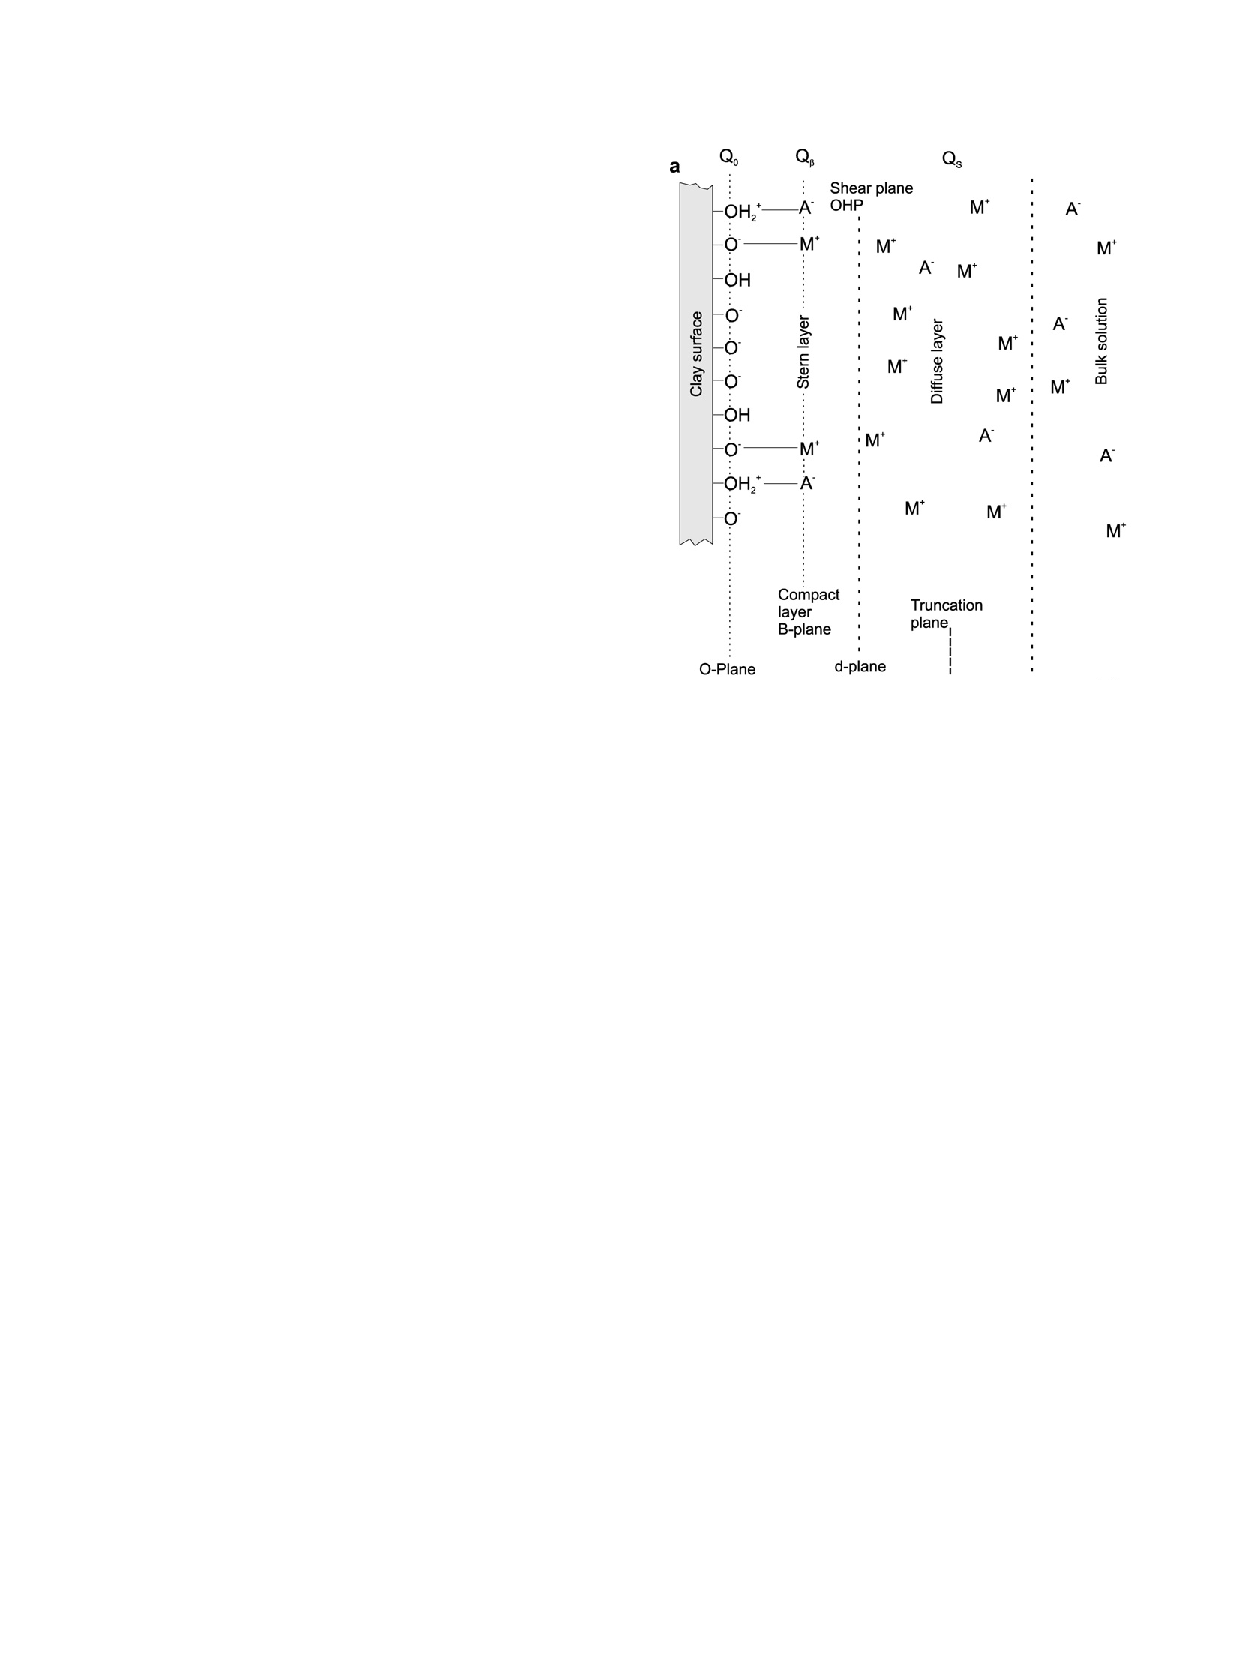
\includegraphics[width=0.75\linewidth]
                    {figs/sorption/goncalves-2007-TLM-Fig-a.pdf}
    \\[24pt]
    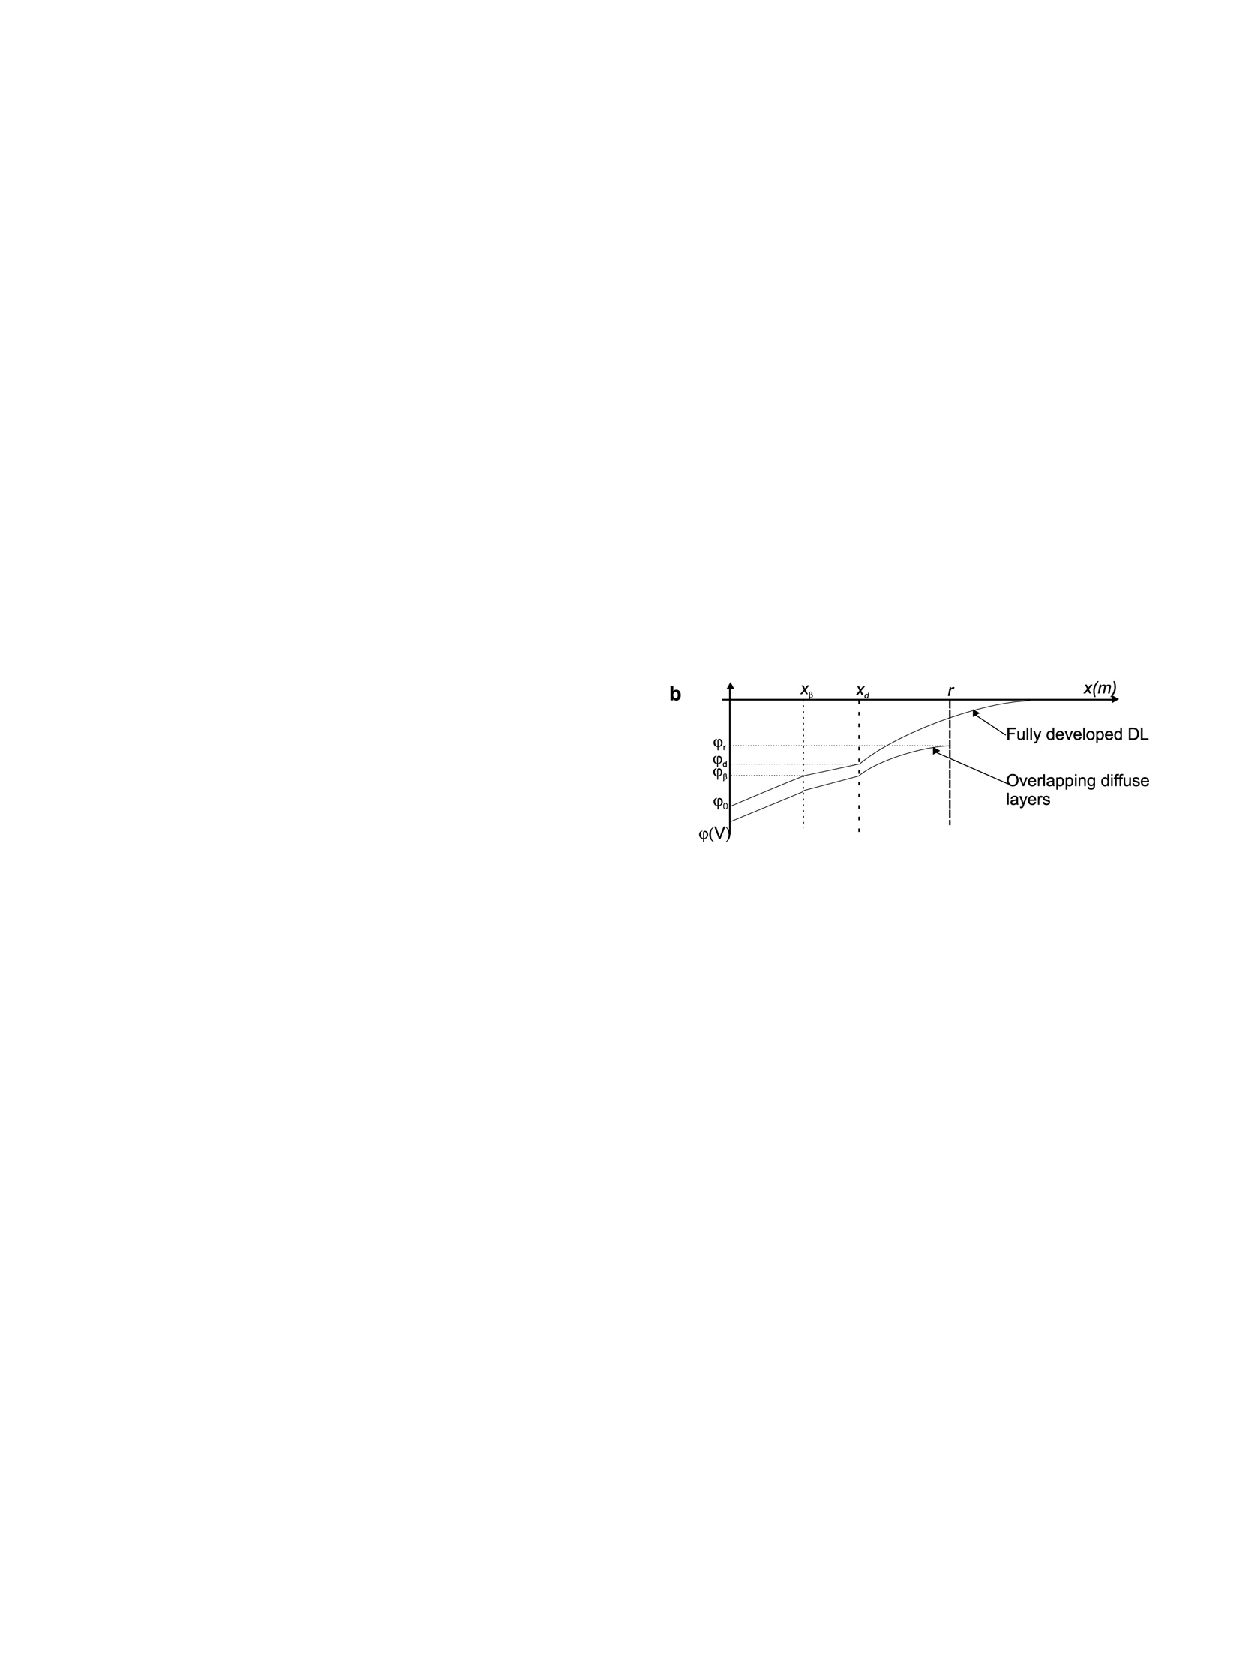
\includegraphics[width=0.75\linewidth]
                    {figs/sorption/goncalves-2007-TLM-Fig-b.pdf}
  \end{center} 
  \caption{Schematic of the TLM model from \citet{goncalves-2007}.}    
  \label{fig:triple-layer-model}
\end{figure}

\end{enumerate}
%  End electrostatic models

\end{enumerate}
%  End sub-models

\subsubsection{Common Data Needs for Sorption Models}
%\todo{Need to gather more requirements for this}

All sorption models will require access to a database of parameter values that are potentially independent of the specific contaminated site under consideration.  For example, the cation exchange capacity (CEC) of a mineral like smectite or kaolinite can be described with a range of values.  However, it is likely that site-specific experimental data will have to
be collected and either collected in a site-specific database, or serve as the basis of a site-specific lookup table.

%\todo{Davis: A database for Freundlich parameters is required? Is
% there such a database? In general, I think the model requirements
% for Kd, Langmuir, Freundlich, surface complexation and ion exchange
%  should state that it is likeley that experimental data have to be
%  collected with site-specific samples.}

